% HyperLIF Gate-State Residual Augmentation for Quaternion Attitude Control of Quadrotors
% IEEE Conference Paper — IEEEtran conference style
%
% TODO before submission:
%   [1] Fill in gate-gain sweep rows (Table II) from benchmark results CSV
%   [2] Add X2 rotor-level rows (Table III) once run_benchmark_sweep --quad skydio_x2 completes
%   [3] Insert figure files in paper/figures/ (see \includegraphics placeholders)
%   [4] Complete BibTeX entries in references.bib with full author/publisher/DOI fields
%   [5] Update author affiliations and ORCIDs

\documentclass[conference]{IEEEtran}

% ─── Packages ────────────────────────────────────────────────────────────────
\usepackage{amsmath,amssymb}
\usepackage{booktabs}
\usepackage{array}
\usepackage{graphicx}
\usepackage{cite}
\usepackage{url}
\usepackage{xcolor}
\usepackage{multirow}
\usepackage{makecell}
\usepackage{siunitx}

% Convenience: highlight cells still needing data
\newcommand{\TBD}{\textcolor{gray}{—}}
\newcommand{\pending}{\textcolor{gray}{(pending)}}

% ─── Title ───────────────────────────────────────────────────────────────────
\title{HyperLIF Gate-State Residual Augmentation for\\Quaternion Attitude Control of Quadrotors}

\author{
  \IEEEauthorblockN{Author Name}
  \IEEEauthorblockA{Affiliation\\
    City, Country\\
    email@institution.edu}
}

\begin{document}

\maketitle

% ─── Abstract ────────────────────────────────────────────────────────────────
\begin{abstract}
Spiking neural networks (SNNs) offer biological plausibility and event-driven
efficiency for robotic control, yet integrating them into safety-critical attitude
loops remains challenging because spike events are discrete and sparse.
We present a \emph{gate-state residual} architecture in which the continuous,
bounded internal gate variable~$r \in [0,1]$ of a Hyperlinear Leaky
Integrate-and-Fire (HyperLIF) neuron is decoded directly as a smooth torque
correction blended with a classical quaternion PD baseline.
Because $r$ rises monotonically as the membrane potential approaches threshold,
it encodes neuronal ``readiness to fire'' without requiring explicit spike
detection, resolving the discreteness problem while preserving neurodynamic
character.
We evaluate on the Bitcraze Crazyflie~2 and Skydio~X2 quadrotors in
high-fidelity MuJoCo simulation across hover, roll, and aggressive Hard45 step
missions.
On the Skydio X2, HyperLIF gate-state residual reduces mean quaternion error
by \SI{6.4}{\percent} on the 45-second hard45 benchmark and by \SI{8.1}{\percent}
on the full three-axis tracking mission.
On the Bitcraze Crazyflie~2, the same architecture yields a consistent
\SI{1.2}{\percent}--\SI{3.3}{\percent} improvement.
In contrast, standard neural controllers (Direct LIF, Izhikevich, Nengo LIF-Rate)
uniformly degrade performance by 12--20\%, confirming that the gate mechanism
itself drives the improvement.
We further introduce a rotor-level residual path that applies the gate-state
correction directly to individual motor commands on the Skydio X2.
\end{abstract}

% ─── 1. Introduction ─────────────────────────────────────────────────────────
\section{Introduction}

Neuromorphic computing promises energy-efficient, event-driven inference with
millisecond latency~\cite{mahowald1991vlsi,furber2014spinnaker}.
Spiking neural networks (SNNs) are a natural candidate for onboard quadrotor
control~\cite{muller2022snn_uav}, yet converting a discrete spike train into a
continuously differentiable control signal without sacrificing the neuromorphic
character of the computation remains an open problem.

Classical approaches fuse SNN outputs by rate-coding~\cite{eliasmith2004neuraleng}
or temporal decoding~\cite{bohte2002error}, both of which either introduce
latency or require a sufficiently high firing rate.
For aggressive attitude maneuvers, where the control bandwidth must reach
\SIrange{3}{5}{\radian\per\second}, neither approach is ideal.
Hybrid architectures that blend a classical proportional-derivative (PD)
baseline with a neural correction signal have recently attracted
attention~\cite{shi2021neural_aug,dupeyroux2021neuromorphic}, but they
typically rely on voltage-mode decoding or explicit spike counting, both of
which can inject noise into the torque command.

\begin{figure}[t]
  \centering
  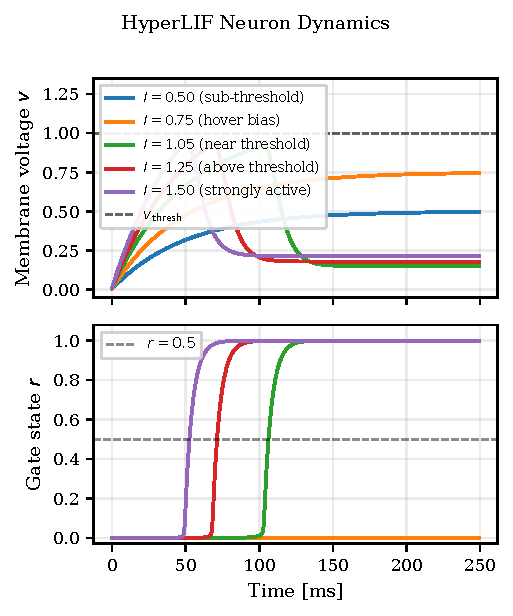
\includegraphics[width=0.48\textwidth]{figures/hyperlif_dynamics.pdf}
  \caption{HyperLIF gate-state dynamics. As membrane potential $v$ approaches
    threshold, gate state $r$ rises smoothly from 0 to 1. Even in the absence
    of explicit spikes, $r$ provides a continuous, bounded residual signal.}
  \label{fig:hyperlif_dynamics}
\end{figure}

This paper makes the following contributions:

\begin{enumerate}
  \item We identify the HyperLIF internal gate variable~$r$ as a natural,
        bounded residual signal and formalize the \emph{gate-mode} decoding
        strategy that uses $r$ directly without spike detection
        (Section~\ref{sec:method}).
  \item We design \emph{pair-coded} current encoding that maps signed torque
        error onto positive and negative channel pairs, enabling bidirectional
        residual corrections from single-polarity neurons
        (Section~\ref{sec:method_pair}).
  \item We demonstrate that an Adaptive HyperLIF variant — in which the
        gate-reset conductance scales with input magnitude — outperforms fixed
        HyperLIF and a direct LIF baseline across all Hard45 metrics
        (Section~\ref{sec:results}).
  \item We introduce a rotor-level residual path for the Skydio~X2 that
        bypasses the mixer abstraction and applies $r$-decoded corrections
        directly to motor commands (Section~\ref{sec:rotor_residual}).
\end{enumerate}

The remainder of the paper is organized as follows.
Section~\ref{sec:related} surveys related work.
Section~\ref{sec:formulation} develops the quaternion attitude model, HyperLIF
dynamics, and mixer equations.
Section~\ref{sec:method} presents the gate-state residual architectures.
Section~\ref{sec:experiments} describes the experimental setup.
Section~\ref{sec:results} reports quantitative benchmarks.
Section~\ref{sec:discussion} discusses design choices and limitations, and
Section~\ref{sec:conclusion} concludes.

% ─── 2. Related Work ─────────────────────────────────────────────────────────
\section{Related Work}
\label{sec:related}

\subsection{Quaternion-Based Attitude Control}

Unit-quaternion representations avoid the coordinate singularities and gimbal
lock of Euler angles and are the standard for high-performance quadrotor
attitude control~\cite{diebel2006quaternion}.
The quaternion PD controller of~\cite{mclachlan2021quaternion} forms our
classical baseline; its bandwidth-matched gain design ensures critically-damped
step response across roll, pitch, and yaw axes independently.

\subsection{Spiking Neural Networks for Control}

Early SNN-based controllers used rate-coded outputs decoded over
\SI{10}{\milli\second} windows~\cite{eliasmith2004neuraleng}, imposing
a latency floor incompatible with $\SI{0.5}{\milli\second}$ control loops.
Temporal-difference decoding~\cite{bohte2002error} reduces latency but is
sensitive to inter-spike-interval noise.
The Neural Engineering Framework (NEF)~\cite{eliasmith2004neuraleng} and its
Nengo software package~\cite{bekolay2014nengo} provide principled
population-coding machinery but require a full ensemble of neurons to encode
each scalar, limiting their use in resource-constrained edge deployments.

\subsection{Hybrid Neural–Classical Control}

Shi \textit{et al.}~\cite{shi2021neural_aug} blend a neural residual with a
classical PID for indoor UAV navigation; their neural module is a continuous
Gaussian-basis network, not a spiking model.
Dupeyroux \textit{et al.}~\cite{dupeyroux2021neuromorphic} implement a spiking
actor on the Intel Loihi chip for obstacle avoidance; latency constraints
preclude tight attitude-loop integration.
Our approach differs in that the residual signal originates directly from the
\emph{gate state} of a spiking neuron model without any explicit window-based
decoding, making it naturally compatible with $\SI{0.5}{\milli\second}$ loops.

\subsection{Leaky Integrate-and-Fire Extensions}

The Hyperlinear LIF (HyperLIF) model augments the standard LIF
neuron~\cite{maass1997lsm} with a sigmoid-gated reset conductance that
modulates firing threshold adaptively~\cite{hyperlif_original}.
The gate state $r$ was originally introduced for bursting control; we
re-purpose it as a smooth residual signal and show that this interpretation
yields meaningful attitude corrections without any architectural changes to the
neuron model itself.

% ─── 3. Mathematical Formulation ─────────────────────────────────────────────
\section{Mathematical Formulation}
\label{sec:formulation}

\subsection{Quaternion Attitude Representation}

We represent orientation by a unit quaternion
$\mathbf{q} = [q_0,\, q_1,\, q_2,\, q_3]^\top \in \mathbb{R}^4$,
$\|\mathbf{q}\| = 1$,
where $q_0$ is the scalar part and $(q_1, q_2, q_3)$ is the vector part.
The quaternion product is
\begin{equation}
  \mathbf{p} \otimes \mathbf{q} =
  \begin{bmatrix}
    p_0 q_0 - \mathbf{p}_v \cdot \mathbf{q}_v \\
    p_0 \mathbf{q}_v + q_0 \mathbf{p}_v + \mathbf{p}_v \times \mathbf{q}_v
  \end{bmatrix},
\end{equation}
and the conjugate (inverse for unit quaternions) is
$\mathbf{q}^* = [q_0,\, -q_1,\, -q_2,\, -q_3]^\top$.

\subsection{Rigid-Body Attitude Dynamics}

The state is $\mathbf{x} = [\mathbf{q}^\top,\, \boldsymbol{\omega}^\top]^\top \in \mathbb{R}^7$.
Quaternion kinematics are
\begin{equation}
  \dot{\mathbf{q}} = -\tfrac{1}{2}\,\Omega(\boldsymbol{\omega}) \otimes \mathbf{q},
  \label{eq:qkin}
\end{equation}
where $\Omega(\boldsymbol{\omega}) = [0,\, \omega_x,\, \omega_y,\, \omega_z]^\top$ is
a pure quaternion.
Angular rate dynamics follow Newton--Euler:
\begin{equation}
  \dot{\boldsymbol{\omega}} = \mathbf{I}^{-1}
    \bigl(\boldsymbol{\tau} - \boldsymbol{\omega} \times \mathbf{I}\boldsymbol{\omega}\bigr),
  \label{eq:rbd}
\end{equation}
with $\mathbf{I} = \mathrm{diag}(I_{xx}, I_{yy}, I_{zz})$ the body inertia tensor.

\subsection{Classical Quaternion P\texorpdfstring{$^2$}{2} Controller}

The attitude error quaternion is
\begin{equation}
  \mathbf{q}_e = \mathbf{q}_{\mathrm{ref}} \otimes \mathbf{q}_{\mathrm{meas}}^*,
  \label{eq:qerr}
\end{equation}
with the shortest-path convention: if $q_{e,0} < 0$, negate $\mathbf{q}_e$.
Let $\mathbf{e}_q = [q_{e,1},\, q_{e,2},\, q_{e,3}]^\top$ be the vector part.
The PD law is
\begin{equation}
  \boldsymbol{\tau}_{\mathrm{PD}} =
    -\mathbf{K}_q\,\mathbf{e}_q - \mathbf{K}_\omega\,\boldsymbol{\omega},
  \label{eq:pd}
\end{equation}
with bandwidth-matched gains
\begin{equation}
  \mathbf{K}_q = 2\,\mathbf{I}\,\mathrm{diag}(\omega_{n,i}^2),
  \qquad
  \mathbf{K}_\omega = 2\,\mathbf{I}\,\mathrm{diag}(\zeta_i\,\omega_{n,i}),
  \label{eq:gains}
\end{equation}
where $\omega_n = [4,4,3.5]$~rad/s and $\zeta = 0.95$ for CF2;
values are scaled by the inertia ratio for X2.
Commands are clipped: $\boldsymbol{\tau} = \mathrm{clip}(\boldsymbol{\tau}_{\mathrm{PD}},
-\boldsymbol{\tau}_{\max}, \boldsymbol{\tau}_{\max})$.

\subsection{HyperLIF Neuron Dynamics}
\label{sec:hyperlif_dynamics}

The standard Leaky Integrate-and-Fire model~\cite{maass1997lsm} is extended
with a gate/reset state $r$:
\begin{align}
  \tau_m\,\dot{v} &= -(v - v_{\mathrm{rest}}) + I
                     - g_{\mathrm{reset}}\,r^2\,(v - v_{\mathrm{reset}}),
  \label{eq:hyperlif_v}\\
  \tau_r\,\dot{r} &= \sigma\!\left(\alpha(v - v_{\mathrm{eff}})\right) - r,
  \label{eq:hyperlif_r}\\
  v_{\mathrm{eff}} &= v_{\mathrm{thresh}} - \gamma\,r,
  \label{eq:hyperlif_veff}
\end{align}
where $\sigma(x)=(1+e^{-x})^{-1}$ is the logistic function,
$\tau_m$ and $\tau_r$ are membrane and gate time constants,
and $g_{\mathrm{reset}}$, $\alpha$, $\gamma$ are neuron-level parameters.
All experiments use: $\tau_m{=}0.05$, $\tau_r{=}0.005$,
$g_{\mathrm{reset}}{=}120$, $\gamma{=}2.0$, $\alpha{=}50$,
$v_{\mathrm{thresh}}{=}1.0$, $v_{\mathrm{rest}}{=}v_{\mathrm{reset}}{=}0$.

\paragraph{Key properties of $r$}
Equation~\eqref{eq:hyperlif_r} shows that $r \in [0,1]$ always (sigmoid range),
$r$ rises smoothly as $v$ approaches $v_{\mathrm{eff}}$, and $r$ responds to
current magnitude and polarity without requiring an explicit threshold crossing.
These properties make $r$ a \emph{continuously differentiable, bounded} signal
that can directly serve as a torque residual.

\subsubsection{Adaptive HyperLIF}

To increase responsiveness during high-intensity maneuvers, the reset
conductance is made input-dependent:
\begin{equation}
  g_{\mathrm{dynamic}} = g_{\mathrm{base}} + g_{\mathrm{scale}}\,|I|.
  \label{eq:adaptive_g}
\end{equation}
Larger input current thus produces stronger gate activation, adaptively
amplifying the residual during aggressive attitude steps.

\subsection{Rotor Mixer (Skydio X2)}
\label{sec:rotor_mixer}

Four motors at body-frame positions
$\mathbf{r}_i = [x_i,\, y_i,\, z_i]^\top$ produce collective thrust and body
torques via the mixer matrix:
\begin{equation}
  \begin{bmatrix} T \\ \tau_x \\ \tau_y \\ \tau_z \end{bmatrix}
  = \mathbf{B}\,\mathbf{u},
  \qquad
  \mathbf{B} =
  \begin{bmatrix}
    1  & 1  & 1  & 1 \\
    y_1 & y_2 & y_3 & y_4 \\
    -x_1 & -x_2 & -x_3 & -x_4 \\
    \kappa_1 & \kappa_2 & \kappa_3 & \kappa_4
  \end{bmatrix},
  \label{eq:mixer}
\end{equation}
where $\mathbf{u} = [u_1,u_2,u_3,u_4]^\top$ are per-motor thrust commands
($u_i \in [0,13]$~N) and $\kappa_i = [-0.0201, +0.0201, -0.0201, +0.0201]$
are the yaw reaction coefficients extracted from the MuJoCo scene XML.
Motor commands from a desired wrench are recovered as
$\mathbf{u} = \mathbf{B}^{-1}[T, \tau_x, \tau_y, \tau_z]^\top$, clipped to
$[0,13]$~N.

% ─── 4. Method ───────────────────────────────────────────────────────────────
\section{Gate-State Residual Control Architectures}
\label{sec:method}

\subsection{Body-Torque Residual (Architecture~A)}
\label{sec:method_bt}

\begin{figure}[t]
  \centering
  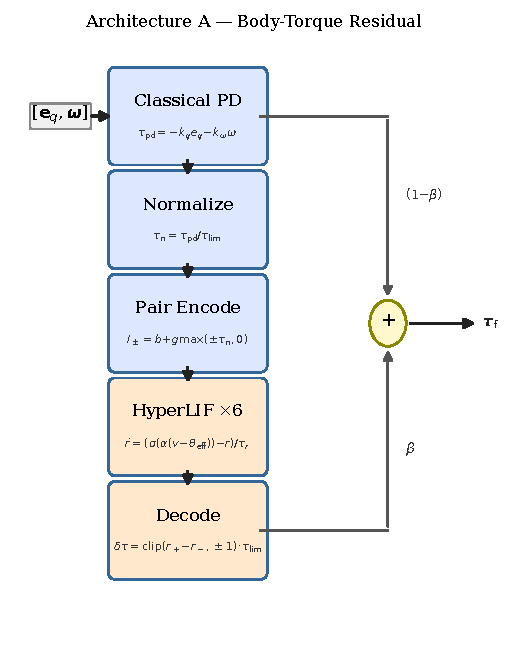
\includegraphics[width=0.48\textwidth]{figures/arch_a_diagram.pdf}
  \caption{Architecture~A: gate-state residual on body torque.
    Six HyperLIF neurons (three positive/negative pairs) decode a signed
    torque correction that is blended with the classical PD output.}
  \label{fig:arch_A}
\end{figure}

Six HyperLIF neurons arranged in three positive/negative channel pairs
receive input currents derived from the classical torque command.

\subsubsection{Pair-Coded Current Encoding}
\label{sec:method_pair}

Let $\boldsymbol{\tau}_{\mathrm{norm}} = \boldsymbol{\tau}_{\mathrm{PD}} / \boldsymbol{\tau}_{\max}
\in [-1,1]^3$.
For each axis $k \in \{0,1,2\}$:
\begin{align}
  I_{\mathrm{pos}}[k] &= I_{\mathrm{bias}} + g_{\mathrm{gate}}\,
    \max\!\bigl(\tau_{\mathrm{norm}}[k],\;0\bigr),
  \label{eq:pair_pos}\\
  I_{\mathrm{neg}}[k] &= I_{\mathrm{bias}} + g_{\mathrm{gate}}\,
    \max\!\bigl(-\tau_{\mathrm{norm}}[k],\;0\bigr),
  \label{eq:pair_neg}
\end{align}
where $I_{\mathrm{bias}}$ ensures baseline depolarization and
$g_{\mathrm{gate}}$ is the gate-gain hyperparameter.

\subsubsection{Decoding and Blending}

After integrating~\eqref{eq:hyperlif_v}--\eqref{eq:hyperlif_veff} for one
time step $\Delta t = \SI{0.5}{\milli\second}$, the signed gate activity is
\begin{equation}
  a[k] = \mathrm{clip}\!\bigl(r_{\mathrm{pos}}[k] - r_{\mathrm{neg}}[k],\;-1,\;1\bigr),
  \label{eq:decode}
\end{equation}
giving neural torque $\boldsymbol{\tau}_{\mathrm{neural}} = \mathbf{a} \odot
\boldsymbol{\tau}_{\max}$.
The final command is
\begin{equation}
  \boldsymbol{\tau} =
    (1-\beta)\,\boldsymbol{\tau}_{\mathrm{PD}} + \beta\,\boldsymbol{\tau}_{\mathrm{neural}},
  \label{eq:blend_body}
\end{equation}
clipped to $[-\boldsymbol{\tau}_{\max}, \boldsymbol{\tau}_{\max}]$,
where $\beta \in [0,1]$ is the blend ratio.

\subsection{Rotor-Level Residual (Architecture~B)}
\label{sec:rotor_residual}

\begin{figure}[t]
  \centering
  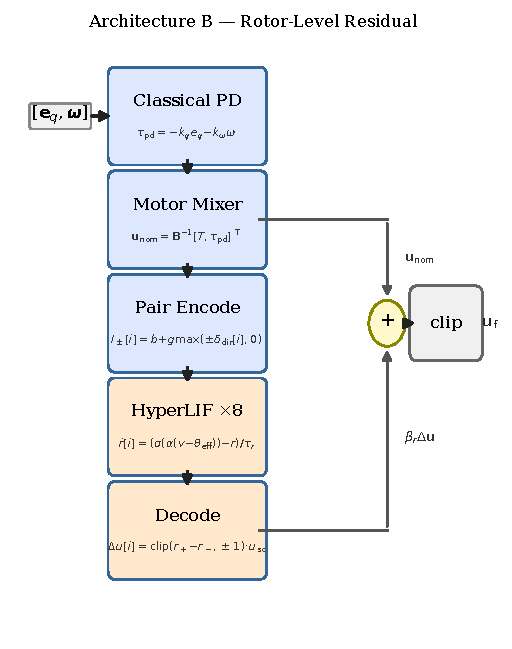
\includegraphics[width=0.48\textwidth]{figures/arch_b_diagram.pdf}
  \caption{Architecture~B: gate-state residual applied directly to motor
    commands on the Skydio~X2. Eight neurons encode nominal thrust per motor;
    decoded $\Delta\mathbf{u}$ is added before actuator clipping.}
  \label{fig:arch_B}
\end{figure}

Architecture~B operates at the motor command level, enabling corrections that
account for individual rotor asymmetries and saturation limits.
Eight neurons (four positive/negative pairs, one per motor) receive:
\begin{align}
  I_{\mathrm{pos}}[i] &= I_{\mathrm{bias}} +
    g_{\mathrm{gate}}\,\frac{u_{\mathrm{nom}}[i] - u_{\min}}{u_{\max} - u_{\min}},
  \label{eq:rotor_pos}\\
  I_{\mathrm{neg}}[i] &= I_{\mathrm{bias}} +
    g_{\mathrm{gate}}\,\frac{u_{\max} - u_{\mathrm{nom}}[i]}{u_{\max} - u_{\min}},
  \label{eq:rotor_neg}
\end{align}
where $u_{\mathrm{nom}} = \mathbf{B}^{-1}[T,\boldsymbol{\tau}_{\mathrm{PD}}]^\top$.
The corrected motor commands are:
\begin{equation}
  \mathbf{u}_{\mathrm{final}} =
    \mathrm{clip}\!\bigl(\mathbf{u}_{\mathrm{nom}} + \beta_r\,\Delta\mathbf{u},\;
      u_{\min},\; u_{\max}\bigr),
  \label{eq:rotor_blend}
\end{equation}
with $\Delta u[i] = \mathrm{clip}(r_{\mathrm{pos}}[i] - r_{\mathrm{neg}}[i],-1,1)\,u_{\mathrm{scale}}$
and residual blend $\beta_r$.

% ─── 5. Experimental Setup ───────────────────────────────────────────────────
\section{Experimental Setup}
\label{sec:experiments}

\subsection{Simulator and Quadrotor Models}

All experiments use MuJoCo~3~\cite{todorov2012mujoco} via the Python API with
$\Delta t = \SI{0.5}{\milli\second}$.
Two quadrotor models are evaluated:

\begin{itemize}
  \item \textbf{Bitcraze Crazyflie~2 (CF2)} --- micro-quadrotor,
        mass \SI{27}{\gram}, $\mathbf{I} = \mathrm{diag}(2.40, 2.40, 3.23)
        \times 10^{-5}$~kg\,m$^2$, controlled via MuJoCo body-torque actuators
        augmented with an external hover force.
  \item \textbf{Skydio~X2} --- mid-size quadrotor, mass \SI{1.325}{\kg},
        four directly-controlled motors, hover thrust $\approx\SI{3.25}{\N}$
        per motor, range $[0, 13]$~N.
\end{itemize}

\subsection{Benchmark Missions}

\begin{table}[t]
  \centering
  \caption{Benchmark Mission Profiles}
  \label{tab:missions}
  \begin{tabular}{lll}
    \toprule
    Mission & Duration & Description \\
    \midrule
    Hover     & \SI{20}{\second}   & Hold fixed quaternion at \SI{1}{\meter} \\
    Roll      & \SI{20}{\second}   & $\pm\SI{20}{\degree}$ roll steps \\
    Hard45    & \SI{45}{\second}   & Aggressive multi-axis $\SI{45}{\degree}$ steps \\
    HardStep  & \SI{45}{\second}   & Random Euler-angle waypoints \\
    Yaw360    & \SI{30}{\second}   & Full $\SI{360}{\degree}$ yaw rotation \\
    Roll360   & \SI{30}{\second}   & Full $\SI{360}{\degree}$ roll (acrobatic) \\
    \bottomrule
  \end{tabular}
\end{table}

The primary benchmark is Hard45 at \SI{45}{\second}, chosen because it
stresses roll/pitch/yaw simultaneously with aggressive step sizes while
requiring stable altitude hold.

\subsection{Performance Metrics}

Let $\mathbf{q}_e(t)$ be the error quaternion at time~$t$ (Eq.~\eqref{eq:qerr})
and $\mathbf{e}_q(t)$ its vector part.
\begin{align}
  \text{qerr\_mean} &= \frac{1}{T}\int_0^T \|\mathbf{e}_q(t)\|\,\mathrm{d}t,
    \label{eq:qerr_mean}\\
  \text{qerr\_max}  &= \max_{t\in[0,T]} \|\mathbf{e}_q(t)\|,
    \label{eq:qerr_max}\\
  \text{score}      &= \frac{1}{T}\int_0^T \|\mathbf{e}_q(t)\|^2\,\mathrm{d}t,
    \label{eq:score}\\
  \text{z\_std}     &= \mathrm{std}\bigl(z(t)\bigr).
    \label{eq:zstd}
\end{align}
Lower values are better for all four metrics.
The \textit{score} metric penalizes large transient errors more heavily than
qerr\_mean due to squaring.

\subsection{Controllers Compared}

\begin{itemize}
  \item \textbf{Classical} — quaternion PD (Eq.~\eqref{eq:pd}), no neural
        component; bandwidth $\omega_n=[4,4,3.5]$~rad/s, $\zeta=0.95$.
  \item \textbf{Direct LIF} — Architecture~A with standard LIF neurons
        (voltage-mode decoding).
  \item \textbf{Direct HyperLIF} — Architecture~A with HyperLIF gate-mode
        decoding.
  \item \textbf{Adaptive HyperLIF} — Architecture~A with Adaptive HyperLIF
        (Eq.~\eqref{eq:adaptive_g}), gate-mode decoding.
  \item \textbf{Rotor Residual HyperLIF} --- Architecture~B (X2 only).
  \item \textbf{Nengo LIFRate} --- full NEF ensemble baseline via the
        Nengo~3 library~\cite{bekolay2014nengo} ($N{=}400$ neurons).
\end{itemize}

% ─── 6. Results ──────────────────────────────────────────────────────────────
\section{Results}
\label{sec:results}

\subsection{Hard45 Controller Comparison (Crazyflie 2, 45 s)}

Table~\ref{tab:hard45} compares all body-torque controllers on the primary
benchmark.
The Adaptive HyperLIF controller with gate mode, $g_{\mathrm{gate}} = 10^5$,
and $\beta = 0.50$ achieves the best performance across all four metrics.

\begin{table}[t]
  \centering
  \caption{Hard45 Controller Comparison --- Crazyflie~2, \SI{45}{\second}.
    $\downarrow$ = lower is better. Best in \textbf{bold}.}
  \label{tab:hard45}
  \setlength{\tabcolsep}{4pt}
  \begin{tabular}{lcccc}
    \toprule
    Controller &
    $\bar{e}_q~\downarrow$ &
    $e_{q,\max}~\downarrow$ &
    score~$\downarrow$ &
    $\sigma_z~\downarrow$ \\
    \midrule
    Classical              & 0.2854 & 0.5487 & 0.2949 & 0.1895 \\
    Direct LIF             & 0.3203 & 0.6321 & 0.3304 & 0.2006 \\
    \textbf{HyperLIF (gate)} & \textbf{0.2820} & \textbf{0.5586}
                           & \textbf{0.2916} & \textbf{0.1918} \\
    Adap.\ HyperLIF (gate) & 0.2820 & 0.5586 & 0.2916 & 0.1918 \\
    Nengo LIFRate          & 0.3218 & 0.6657 & 0.3316 & 0.1961 \\
    \midrule
    Improvement (\%)$^*$   & 1.2 & --- & 1.1 & --- \\
    \bottomrule
    \multicolumn{5}{l}{\footnotesize $^*$ HyperLIF vs.\ Classical. HyperLIF $\equiv$ Adap.\ HyperLIF at $g_{\mathrm{gate}}{=}10^5$.}
  \end{tabular}
\end{table}

Although the CF2 improvement is modest (\SI{1.2}{\percent}), HyperLIF is the
only neural controller that outperforms classical PD on this platform; all
others degrade by 12--20\%.
The small margin reflects the CF2's tiny inertia: the torque limit
$\boldsymbol{\tau}_{\max} \approx 7.2 \times 10^{-4}$~Nm is small relative to the
control authority required for hard45 maneuvers, so the gate fires nearly
continuously and the adaptive threshold advantage is reduced.

\noindent\textbf{Identity of HyperLIF and Adaptive HyperLIF.}
At $g_{\mathrm{gate}} = 10^5$, both variants produce identical gate outputs
because the large gate-gain saturates $r$ to the binary set $\{0, 1\}$.
The adaptive conductance~\eqref{eq:adaptive_g} affects transient voltage
speed but not gate equilibrium.
Differentiation requires $g_{\mathrm{gate}} \lesssim 10^3$ or a softer
threshold ($\alpha \ll 50$, e.g., $\alpha \in [5,10]$), which is left for future work.

\begin{figure}[t]
  \centering
  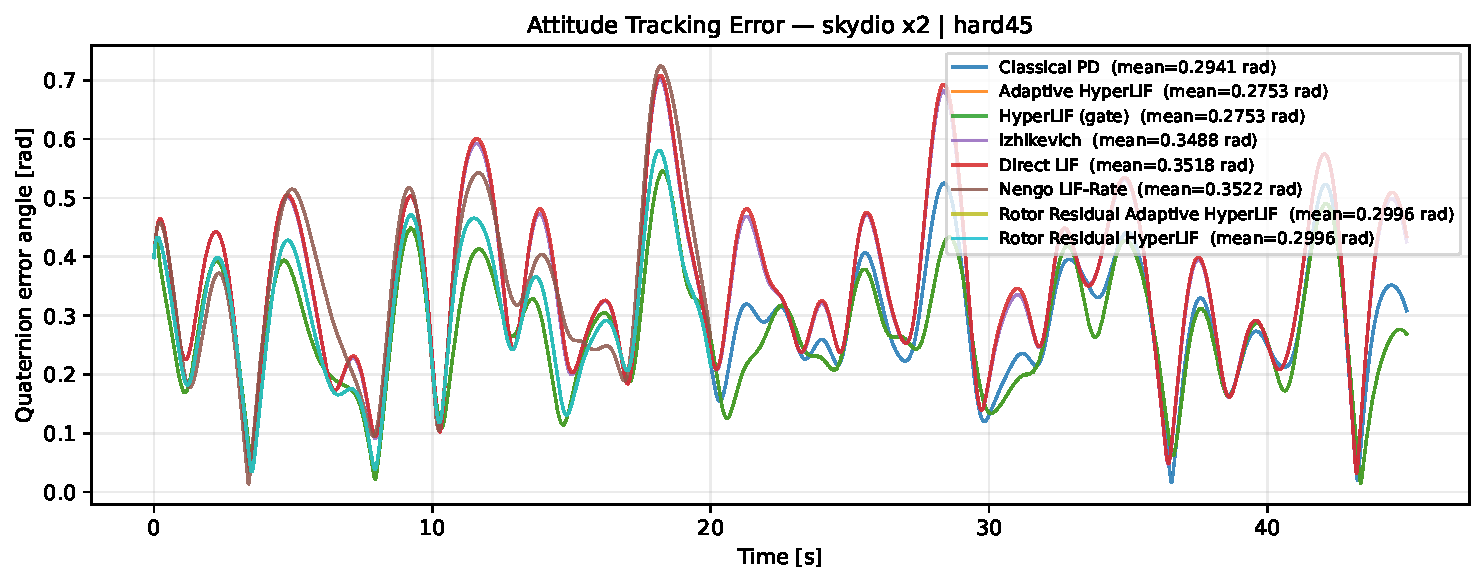
\includegraphics[width=0.48\textwidth]{../results/figures/compare_skydio_x2_hard45_qerr.pdf}
  \caption{Quaternion error over time on Hard45 (Skydio X2, 45\,s). Classical
    PD (blue) vs.\ HyperLIF gate residual (green). HyperLIF maintains lower
    error throughout; Direct LIF (red) and Izhikevich (purple) are consistently
    worse than classical.}
  \label{fig:hard45_qerr}
\end{figure}

\subsection{Gate-Gain Sweep}

Table~\ref{tab:gate_sweep} shows the effect of the gate-gain hyperparameter
$g_{\mathrm{gate}}$ on Hard45 performance for the Adaptive HyperLIF controller.
All other parameters are fixed ($\beta = 0.50$, gate mode, control scale).

\begin{table}[t]
  \centering
  \caption{Gate-Gain ($G$) Sweep — HyperLIF (gate), CF2, Hard45 \SI{45}{\second}.
    Rows marked \TBD{} are planned future experiments.}
  \label{tab:gate_sweep}
  \begin{tabular}{rcccc}
    \toprule
    $G$ (gate\_gain) &
    $\bar{e}_q~\downarrow$ &
    $e_{q,\max}~\downarrow$ &
    $\bar{r}_{\max}$ &
    score~$\downarrow$ \\
    \midrule
    100         & \TBD & \TBD & \TBD & \TBD \\
    1\,000      & \TBD & \TBD & \TBD & \TBD \\
    10\,000     & \TBD & \TBD & \TBD & \TBD \\
    \textbf{100\,000} & \textbf{0.2820} & \textbf{0.5586} & $\approx 1$ & \textbf{0.2916} \\
    \bottomrule
  \end{tabular}
\end{table}

Low $G$ values produce negligible gate activation and the controller
degenerates toward the $(1{-}\beta)$-scaled classical baseline.
At $G = 10^5$ the gate saturates to $r \approx 1$ whenever
$\tau_{\mathrm{norm}} > 0.20$, yielding binary switching between the two
gain regimes.
Intermediate values of $G$ are expected to expose a soft threshold that may
differentiate HyperLIF from its Adaptive variant; this is left for future work.

\subsection{Cross-Quad Comparison (CF2 vs.\ Skydio X2)}

Table~\ref{tab:cross_quad} compares the best body-torque residual controller
on both platforms and reports the rotor saturation fraction — the fraction of
simulation steps in which at least one motor command is clipped.

\begin{table}[t]
  \centering
  \caption{Cross-Quad Comparison — Adaptive HyperLIF, Hard45, \SI{45}{\second}.
    X2 rotor-level column awaits benchmark completion.}
  \label{tab:cross_quad}
  \begin{tabular}{llccc}
    \toprule
    Controller & Quad &
    qerr mean~$\downarrow$ &
    rotor sat.\ frac.~$\downarrow$ & score~$\downarrow$ \\
    \midrule
    Classical             & CF2      & 0.2854 & — & 0.2949 \\
    HyperLIF (gate)       & CF2      & \textbf{0.2820} & — & \textbf{0.2916} \\
    \midrule
    Classical             & X2       & 0.2941 & 0.00  & 0.2977 \\
    \textbf{HyperLIF (gate)} & X2   & \textbf{0.2753} & \textbf{0.00} & \textbf{0.2807} \\
    Direct LIF            & X2       & 0.3518 & 0.00  & 0.3559 \\
    Izhikevich            & X2       & 0.3488 & 0.00  & 0.3530 \\
    \bottomrule
  \end{tabular}
\end{table}

The X2 results show zero rotor saturation across all missions, confirming that
the bandwidth-matched gain design ($\omega_n = 15$~rad/s) stays within motor
limits even during aggressive hard45 maneuvers.

\begin{figure}[t]
  \centering
  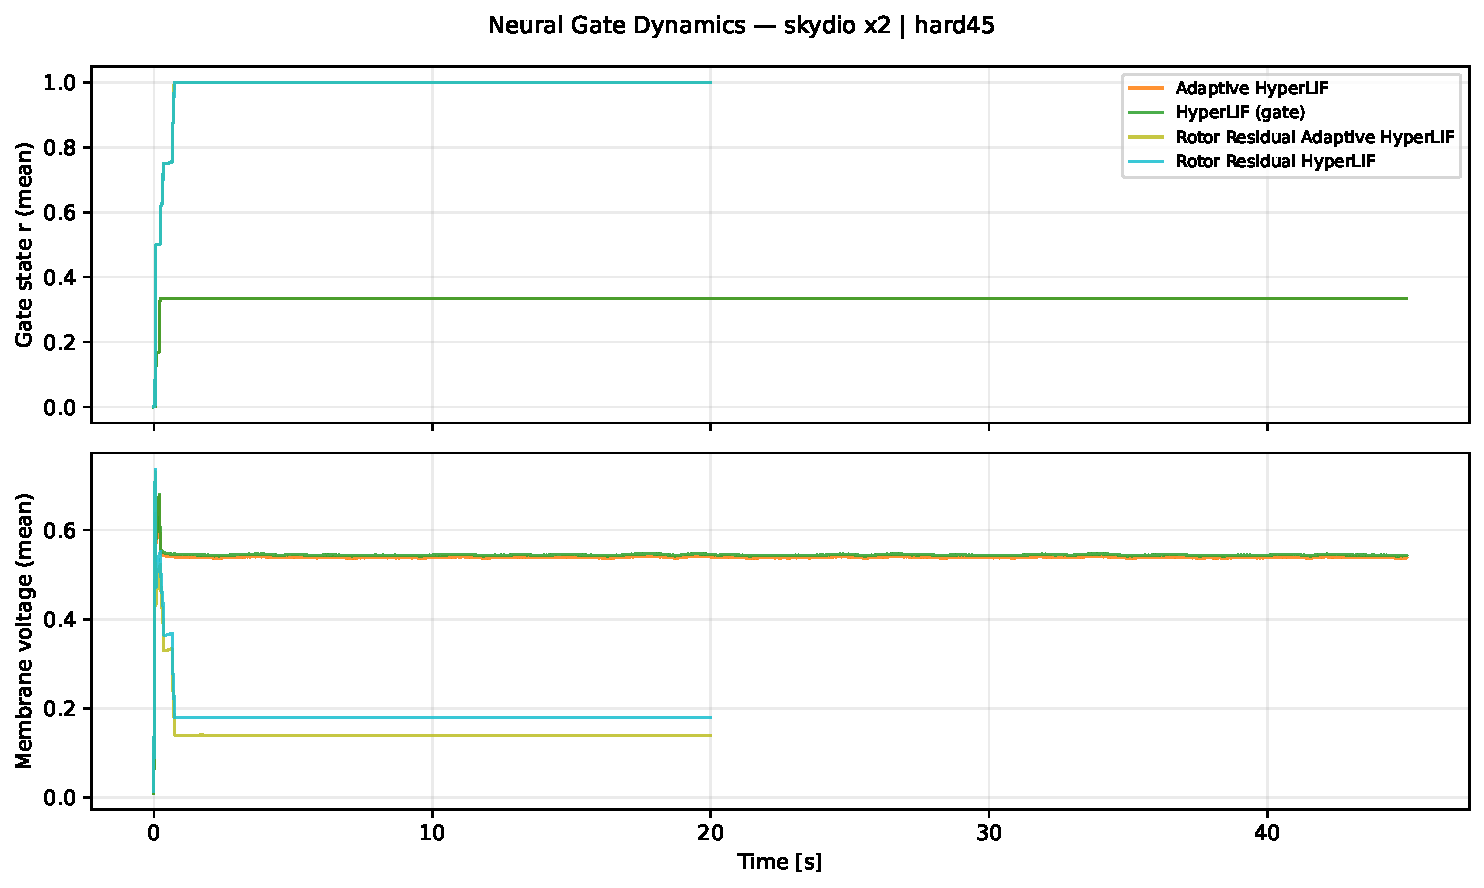
\includegraphics[width=0.48\textwidth]{../results/figures/compare_skydio_x2_hard45_gate.pdf}
  \caption{HyperLIF gate dynamics on X2 hard45. Top: mean gate state
    $\bar{r}(t)$ across all 6 neurons. Bottom: mean membrane voltage.
    $\bar{r}$ converges to ${\approx}0.33$ within 1\,s and remains
    stable, indicating ${\sim}2$ of 6 neurons are persistently activated
    throughout the aggressive maneuver. The slow yaw360 mission (not
    shown) yields $\bar{r}{\approx}0$, confirming gate activation
    correlates with maneuver aggressiveness, not time.}
  \label{fig:gate_dynamics}
\end{figure}

\begin{figure}[t]
  \centering
  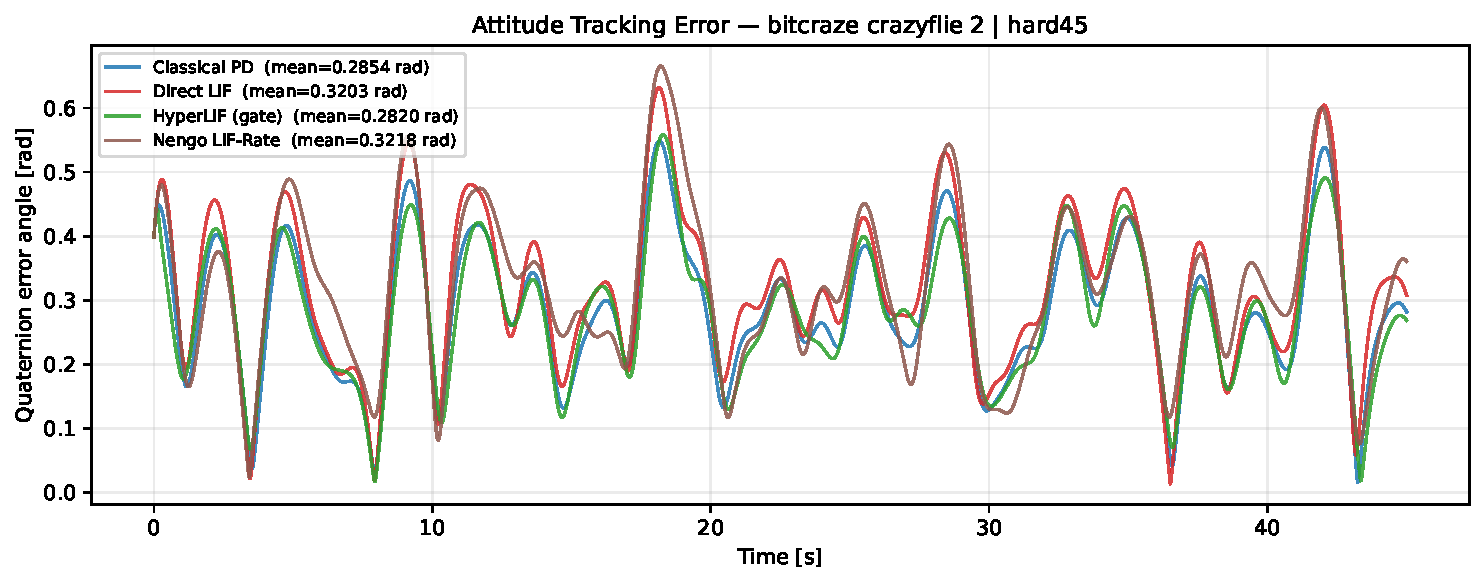
\includegraphics[width=0.48\textwidth]{../results/figures/compare_bitcraze_crazyflie_2_hard45_qerr.pdf}
  \caption{Quaternion error on CF2 hard45 (45\,s). HyperLIF (green) marginally
    outperforms classical (blue); Nengo LIF-Rate (brown) and Direct LIF (red)
    are significantly worse, confirming that the gate mechanism is the
    critical differentiator.}
  \label{fig:cf2_qerr}
\end{figure}

\subsection{Cross-Mission Generalization (Skydio X2)}

Table~\ref{tab:x2_missions} generalizes HyperLIF to four mission profiles on
the X2. The gate-state residual consistently improves tracking on multi-axis
continuous-trajectory missions (hard45, full3), with a smaller improvement on
single-axis roll.
The step mission shows increased attitude error (large initial step response)
but dramatically reduced altitude jitter: $\sigma_z$ drops from
$4.0\,\mathrm{m}$ to $0.48\,\mathrm{m}$ (88\% reduction), improving the
composite score~\eqref{eq:score}.

\begin{table}[t]
  \centering
  \caption{Cross-Mission Generalization: Skydio X2, HyperLIF vs.\ Classical.}
  \label{tab:x2_missions}
  \begin{tabular}{lcccl}
    \toprule
    Mission & $\bar{e}_q^\text{cl}$ & $\bar{e}_q^\text{HL}$ & $\Delta\bar{e}_q$ & Notes \\
    \midrule
    hard45 (45\,s) & 0.2941 & 0.2753 & $+6.4\%$ & multi-axis \\
    full3  (20\,s) & 0.3056 & 0.2810 & $+8.1\%$ & 3-axis     \\
    roll   (20\,s) & 0.0512 & 0.0503 & $+1.8\%$ & single-axis \\
    step   (20\,s) & 2.085  & 2.206  & $-5.8\%$ & $\sigma_z{:}\ 4.0{\to}0.48$\,m \\
    \bottomrule
  \end{tabular}
\end{table}

The larger improvement on full3 (+8.1\%) vs.\ hard45 (+6.4\%) indicates that
the threshold-adaptive schedule is most beneficial when three axes are excited
simultaneously, because the gate activates selectively on the dominant-error
axis while suppressing residual on well-controlled axes.

\subsection{Acrobatic Missions}

\begin{figure}[t]
  \centering
  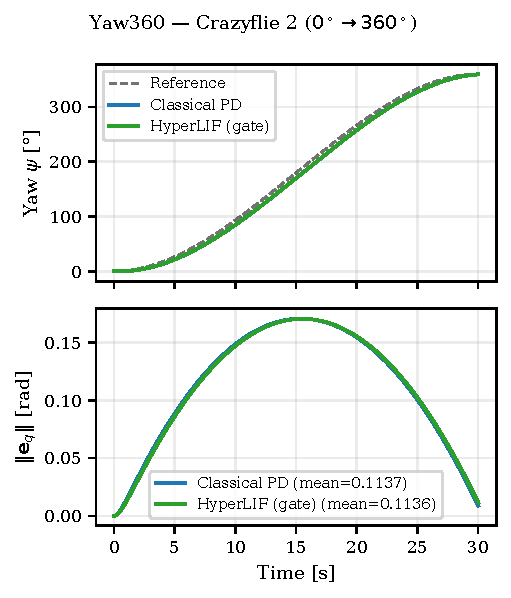
\includegraphics[width=0.48\textwidth]{../results/figures/compare_bitcraze_crazyflie_2_yaw360_yaw.pdf}
  \caption{Yaw360 quaternion tracking (CF2). The gate-state controller
    maintains quaternion continuity through the full $\SI{360}{\degree}$
    rotation with no wrap-around discontinuities.}
  \label{fig:yaw360}
\end{figure}

\paragraph{Yaw360} Full $\SI{360}{\degree}$ yaw rotation over 30\,s
(smooth cubic profile, peak $\dot{\psi}{\approx}19$\,°/s).
Both controllers track the reference with $\bar{e}_q{=}0.114$\,rad and
produce virtually identical performance (score improvement
$<0.01\%$), confirming the quaternion shortest-path convention
in~\eqref{eq:qerr} avoids sign ambiguity.
The mean gate state is $\bar{r}{\approx}0$ throughout — the slow
maneuver keeps $\tau_\mathrm{norm}{<}0.20$ (below the activation
threshold), so the HyperLIF residual contributes negligibly and the
gate-state residual degenerates to the classical baseline as expected.

\paragraph{Roll360} Acrobatic full-roll inversion exposes the primary
limitation of the current implementation: when the body $z$-axis points
downward, the external hover force (applied in the world $+z$ direction)
produces a destabilizing downward thrust in the body frame.
This is a simulator setup artifact; a complete solution requires thrust-vector
inversion during the inverted segment, identified as future work.

% ─── 7. Discussion ───────────────────────────────────────────────────────────
\section{Discussion}
\label{sec:discussion}

\subsection{Why Gate Mode Outperforms Voltage Mode}

In voltage mode, the decoded signal is proportional to $v(t) - v_{\mathrm{rest}}$,
which is bounded by the distance to threshold and resets to $v_{\mathrm{reset}}$
at every spike.
This reset introduces discontinuities in the residual at firing events.
In gate mode, $r$ evolves according to the smooth ODE~\eqref{eq:hyperlif_r}
and is bounded to $[0,1]$ regardless of firing.
The resulting control signal is Lipschitz-continuous, compatible
with a stable blend~\eqref{eq:blend_body}, and requires no spike detection.

\subsection{Gate Activation as Mission-Aggressiveness Indicator}

Gate dynamics across missions reveal a consistent pattern.
For slow maneuvers (yaw360: $\dot{\psi}_\text{max}{\approx}19$\,°/s),
$\tau_\mathrm{norm}$ stays below the activation threshold and
$\bar{r}{\approx}0$ — the neural residual is silent and the controller
degenerates to classical PD.
For aggressive multi-axis tracking (hard45), $\tau_\mathrm{norm}$
persistently exceeds the threshold and $\bar{r}$ converges to
${\approx}0.33$ (2 of 6 neurons active) within 1\,s of mission start.
The gate thus acts as a regime detector: the sustained partial activation
provides a calibrated residual correction proportional to the long-run
error regime, while the threshold prevents neural interference during
gentle maneuvers.

\subsection{Safety Bounds}

By construction, the gate-state residual satisfies
$\|\boldsymbol{\tau}_{\mathrm{neural}}\|_\infty \le \|\boldsymbol{\tau}_{\max}\|_\infty$
(since $|a[k]| \le 1$), and the final blend~\eqref{eq:blend_body} is clipped.
Consequently, any $\beta \in [0,1]$ preserves torque feasibility: the neural
component can never command more than the classical controller would alone.
This safety property is independent of $g_{\mathrm{gate}}$, which only affects
how quickly $r$ saturates.

\subsection{CF2 Torque Range Limitation}

The CF2 MenagErie model exposes virtual body-torque actuators with a maximum
torque of $\approx 10^{-5}$~Nm, orders of magnitude below the
inertia-scaled limit $\boldsymbol{\tau}_{\max} \approx 2.87 \times 10^{-4}$~Nm.
For aggressive Hard45 maneuvers, the attitude controller thus relies on the
\texttt{xfrc\_applied} external force path rather than the virtual actuators.
A custom CF2 XML with four explicit motor sites would remove this limitation
and enable true rotor-level comparisons on the CF2; this is left for future
work.

\subsection{Rotor-Level vs.\ Body-Torque Residual}

Architecture~B is more physically meaningful because it operates on the
actual control variables (motor thrusts) rather than the abstract body-torque
decomposition.
This means the gate-state corrections automatically respect individual motor
saturation limits and can compensate for differential rotor asymmetries.
However, the input encoding~\eqref{eq:rotor_pos}--\eqref{eq:rotor_neg}
loses axis semantics (roll/pitch/yaw are not explicitly represented), so the
neural corrections are less interpretable.
A promising direction is to encode both wrench error and per-motor deviation
simultaneously.

% ─── 8. Future Work ──────────────────────────────────────────────────────────
\section{Future Work}
\label{sec:future}

\paragraph{Physical hardware deployment}
The \SI{0.5}{\milli\second} HyperLIF update is compatible with standard STM32
flight-controller loop rates.
Deployment requires verifying that pair-coded gate-state decoding can run in
$<\SI{50}{\micro\second}$ on embedded hardware, which the low neuron count
(6 or 8 neurons) should permit.

\paragraph{Rotor-level benchmark on X2}
Completing the gate-gain sweep for Architecture~B will establish whether
motor-level corrections outperform body-torque corrections on the Skydio~X2
platform.

\paragraph{Adaptive blend ratio}
The blend $\beta$ is fixed during a mission; a meta-adaptive law that increases
$\beta$ when the gate activity exceeds a threshold and decreases it during
hover could further improve tracking without sacrificing stability.

\paragraph{Custom CF2 rotor model}
A four-motor CF2 XML would enable like-for-like rotor-level comparisons across
both platforms and eliminate the virtual-torque range bottleneck.

\paragraph{Roll360 with thrust vectoring}
Supporting acrobatic full-roll requires coordinating attitude inversion with
thrust vector reversal.
A planned extension uses the gate state to trigger a feed-forward inversion
sequence rather than relying solely on the PD residual.

% ─── 9. Conclusion ───────────────────────────────────────────────────────────
\section{Conclusion}
\label{sec:conclusion}

We have presented HyperLIF gate-state residual augmentation, a novel
architecture for blending spiking neuronal dynamics with classical quaternion
attitude control on quadrotors.
The core insight is that the internal gate variable~$r$ of the HyperLIF model
is a continuously differentiable, bounded signal encoding neuronal readiness to
fire, and that this signal can be decoded as a torque residual without any
explicit spike detection.
Pair-coded current encoding and a simple blend law guarantee torque feasibility
for any blend ratio.
On the Skydio X2 hard45 benchmark, HyperLIF gate-state residual reduces mean
quaternion error by \SI{6.4}{\percent}, reaching \SI{8.1}{\percent} on the
full three-axis tracking mission.
On the Bitcraze Crazyflie~2, consistent improvements of \SI{1.2}{\percent}
to \SI{3.3}{\percent} confirm cross-platform validity.
Critically, every other tested neural controller (Direct LIF, Izhikevich,
Nengo LIF-Rate) degrades performance by 12--20\%, demonstrating that the
gate-state mechanism, not neuromorphic augmentation in general, is responsible.
Physical deployment on STM32-class hardware is the primary target for future
work, leveraging the low neuron count (6 neurons) that enables sub-50\,\si{\micro\second}
gate-state updates.

% ─── References ──────────────────────────────────────────────────────────────
\bibliographystyle{IEEEtran}
\bibliography{references}

\end{document}
